%!TEX root = ../main.tex

\chapter{Machine Learning}\label{cha:machinelearning}

In this chapter a new approach to identifying strategies that are the same will be presented.
A new type of tournament will be presented, and the summary of the results of this tournament will then be used to train a Machine Learning model.
The model is then able to predict whether new strategies are the same as ones already implemented within Axelrod-Python.



\section{Ashlock Tournament}\label{sec:ashlock_tourn}

In an Ashlock tournament, all strategies entered play against a probe strategy for a range of parameters, and do not play each other.
This is similar to how a numerical approximation of a fingerprint is constructed in Chapter \ref{cha:implementation}.
The benefit of this approach is that much more data is collected than just the score of the strategy involved.
Currently in Axelrod-Python, a results file for a tournament includes:

\begin{itemize}
    \item Strategy Name
    \item Rank - Where the strategy ranked overall in the tournament
    \item Median Score
    \item Cooperation Rating
    \item Wins
    \item Initial C rate
    \item CC rate
    \item CD rate
    \item DC rate
    \item DD rate
    \item CC to C rate
    \item CD to C rate
    \item DC to C rate
    \item DD to C rate
\end{itemize}

An example of the results file for strategies that have been played in an Ashlock Tournament is given in Table \ref{tab:ash_results}.

\begin{sidewaystable}[htbp!]
\begin{tabular}{llllllllllHHH}
\toprule
Name &  Median\_score &  Cooperation\_rating &  Wins &  Initial\_C\_rate &  CC\_rate &  CD\_rate &  DC\_rate &  DD\_rate &  CC\_to\_C\_rate &  CD\_to\_C\_rate &  DC\_to\_C\_rate &  DD\_to\_C\_rate \\
\midrule
Defector & 0.59536 & 0.0000 & 22.0 & 0.0 & 0.0000 & 0.0000 & 0.4942 & 0.5058 & 0.0 & 0.0 & 0.0 & 0.0 \\
Win-Stay Lose-Shift & 0.46868 & 0.5528 & 7.0 & 1.0 & 0.3302 & 0.2226 & 0.2264 & 0.2208 & 1.0 & 0.0 & 0.0 & 1.0 \\
Bully & 0.46388 & 0.5024 & 11.0 & 0.0 & 0.1606 & 0.3418 & 0.3350 & 0.1626 & 0.0 & 1.0 & 0.0 & 1.0 \\
Alternator & 0.44824 & 0.5000 &  13.0 & 1.0 & 0.2484 & 0.2516 & 0.2490 & 0.2510 & 0.0 & 0.0 & 1.0 & 1.0 \\
 Tit For Tat & 0.43360 & 0.5144 & 0.0 & 1.0 & 0.3680 & 0.1464 & 0.1446 & 0.3410 & 1.0 & 0.0 & 1.0 & 0.0 \\
\bottomrule
\end{tabular}

\begin{tabular}{lHHHHHHHHHlll}
\toprule
Name &  Median\_score &  Cooperation\_rating &  Wins &  Initial\_C\_rate &  CC\_rate &  CD\_rate &  DC\_rate &  DD\_rate &  CC\_to\_C\_rate &  CD\_to\_C\_rate &  DC\_to\_C\_rate &  DD\_to\_C\_rate \\
\midrule
Defector & 0.59536 & 0.0000 & 22.0 & 0.0 & 0.0000 & 0.0000 & 0.4942 & 0.5058 & 0.0 & 0.0 & 0.0 & 0.0 \\
Win-Stay Lose-Shift & 0.46868 & 0.5528 & 7.0 & 1.0 & 0.3302 & 0.2226 & 0.2264 & 0.2208 & 1.0 & 0.0 & 0.0 & 1.0 \\
Bully & 0.46388 & 0.5024 & 11.0 & 0.0 & 0.1606 & 0.3418 & 0.3350 & 0.1626 & 0.0 & 1.0 & 0.0 & 1.0 \\
Alternator & 0.44824 & 0.5000 &  13.0 & 1.0 & 0.2484 & 0.2516 & 0.2490 & 0.2510 & 0.0 & 0.0 & 1.0 & 1.0 \\
 Tit For Tat & 0.43360 & 0.5144 & 0.0 & 1.0 & 0.3680 & 0.1464 & 0.1446 & 0.3410 & 1.0 & 0.0 & 1.0 & 0.0 \\
\bottomrule
\end{tabular}
\caption{Results of an Ashlock Tournament}
\label{tab:ash_results}

\bigskip

\begin{tabular}{lllllllllHHHHH}
\toprule
Name\_A & Name\_B & Median\_score\_r & Cooperation\_rating\_r & Wins\_r & Initial\_C\_rate\_r & CC\_rate\_r & CD\_rate\_r & DC\_rate\_r & DD\_rate\_r & CC\_to\_C\_rate\_r & CD\_to\_C\_rate\_r & DC\_to\_C\_rate\_r & DD\_to\_C\_rate\_r \\
\midrule
 Defector & Defector & 1.000000 & 1.0 &  1.000000 & 1.0 & 1.0 & 1.0 & 1.000000 & 1.000000 & 1.0 & 1.0 & 1.0 & 1.0 \\
 Defector & Win-Stay Lose-Shift &0.787221 & 0.0 &  0.318182 & 0.0 & 0.0 & 0.0 & 0.458114 & 0.436536 & 0.0 & 1.0 & 1.0 & 0.0 \\
 Defector & Bully & 0.779159 & 0.0 & 0.500000 & 1.0 & 0.0 & 0.0 & 0.677863 & 0.321471 & 1.0 & 0.0 & 1.0 & 0.0 \\
 Defector & Alternator & 0.752889 & 0.0 & 0.590909 & 0.0 & 0.0 & 0.0 & 0.503845 & 0.496244 & 1.0 & 1.0 & 0.0 & 0.0 \\
 Defector & Tit For Tat & 0.728299 & 0.0 &  0.000000 & 0.0 & 0.0 & 0.0 & 0.292594 & 0.674180 & 0.0 & 1.0 & 0.0 & 1.0 \\
\bottomrule
\end{tabular}
\begin{tabular}{llHHHHHHHHllll}
\toprule
Name\_A & Name\_B & Median\_score\_r & Cooperation\_rating\_r & Wins\_r & Initial\_C\_rate\_r & CC\_rate\_r & CD\_rate\_r & DC\_rate\_r & DD\_rate\_r & CC\_to\_C\_rate\_r & CD\_to\_C\_rate\_r & DC\_to\_C\_rate\_r & DD\_to\_C\_rate\_r \\
\midrule
 Defector & Defector & 1.000000 & 1.0 &  1.000000 & 1.0 & 1.0 & 1.0 & 1.000000 & 1.000000 & 1.0 & 1.0 & 1.0 & 1.0 \\
 Defector & Win-Stay Lose-Shift &0.787221 & 0.0 &  0.318182 & 0.0 & 0.0 & 0.0 & 0.458114 & 0.436536 & 0.0 & 1.0 & 1.0 & 0.0 \\
 Defector & Bully & 0.779159 & 0.0 & 0.500000 & 1.0 & 0.0 & 0.0 & 0.677863 & 0.321471 & 1.0 & 0.0 & 1.0 & 0.0 \\
 Defector & Alternator & 0.752889 & 0.0 & 0.590909 & 0.0 & 0.0 & 0.0 & 0.503845 & 0.496244 & 1.0 & 1.0 & 0.0 & 0.0 \\
 Defector & Tit For Tat & 0.728299 & 0.0 &  0.000000 & 0.0 & 0.0 & 0.0 & 0.292594 & 0.674180 & 0.0 & 1.0 & 0.0 & 1.0 \\
\bottomrule
\end{tabular}
\caption{Comparison of the results of an Ashlock Tournament}
\label{tab:ash_comparison}
\end{sidewaystable}



\section{Training the model}\label{sec:training_model}

To train the model, all strategies available in Axelrod-Python were entered into an Ashlock Tournament and a results file was generated, as described in Section \ref{sec:ashlock_tourn}.
Multiple copies of each strategy where included to compensate for the Ashlock Tournament being a stochastic process.
Each copy of a strategy was treated separately and thus had an individual line in the results file.

Once the results had been obtained, a new set of data was created that compared all strategies against each other.
For two strategies $A, B$ with variables $x_i^{(A)}, x_i^{(B)}$, a ratio $r_i^{(A, B)}$ is calculated for each possible variable $x_i$ where:
$$
r_i^{(A, B)} = \frac{\min(x_i^{(A)}, x_i^{(B)})}{\max(x_i^{(A)}, x_i^{(B)})}
$$
In the case where both variable equal zero, instead of the ratio being undefined it is set to 1 to demonstrate that the original variables were equal.
The resulting data is shown in Table \ref{tab:ash_comparison}.
By comparing the names of the two strategies, a new column can be added to the data containing a boolean variable where a value of 1 implies that the two strategies are the same, and 0 if they are different.
This ensures that different copies of the same strategy will still be considered equal.

Figure \ref{fig:ml_process} gives an overview of this process with every colour of \textcolor{sol-violet}{Purple}, \textcolor{sol-red}{Red}, \textcolor{sol-green}{Green} and \textcolor{sol-blue}{Blue} representing a different strategy.
As mentioned previously several copies of each strategy are used which would produce several nodes of the same colour in Figure \ref{fig:ashlock_tourn}, but these have been omitted for clarity.
Likewise, in Figure \ref{fig:model_training} there should be far more rows for each colour but these would clutter the diagram.

Following the diagram from left to right, it begins by playing an Ashlock Tournament as described in Section \ref{sec:ashlock_tourn}.
The results of the the tournament are collected in the next step, and an example of this is given in Table \ref{tab:ash_results}.
In the following stage a new table is created that compares the results of each strategy, again an example is given in Table \ref{tab:ash_comparison}.
Once this table has been created, a sample is taken from all the strategies included in the initial Ashlock Tournament.
Rows from the table containing \textbf{only} these strategies are then used to train the model.
In Figure \ref{fig:ml_process}, the \textcolor{sol-red}{Red} and \textcolor{sol-blue}{Blue} strategies were selected, resulting in rows being selected that contained information relating exclusively to the \textcolor{sol-red}{Red} and \textcolor{sol-blue}{Blue} strategies.
Finally, all remaining rows that were not involved in training the model are collected.
The model is then scored against this unseen data.

\begin{sidewaysfigure}[htbp!]
    \centering
    \subfloat[The Ashlock Tournament]{\includestandalone[width=0.15\textwidth]{../img/AshlockTournament}\label{fig:ashlock_tourn}}
    \subfloat[Training the Model]{\includestandalone[width=0.85\textwidth]{../img/MachineLearningProcess}\label{fig:model_training}}
    \caption{The process for training the Machine Learning Model}
    \label{fig:ml_process}
\end{sidewaysfigure}



\section{Assessing the Model}\label{sec:assessing_model}

The actual Machine Learning was done using the python library \mintinline{python}{sk-learn} \cite{scikit-learn}.
A choice of two models were implemented, Logistic Regression \cite{Schmidt2016, Yu2011} and Support Vector Classification \cite{Smola2004, Vandewalle1999}.
The process for training the models is outlined in Section \ref{sec:training_model} and it is mentioned that a sample must be taken from the strategies used in the initial Ashlock Tournament.
Clearly the larger the sample size, the better the model should perform as it has more data to learn from.
In order to decide whether to use Logistic Regression or SVC, both models were trained/tested against many samples of varying sizes.

Figure \ref{fig:score_4_sample_size} shows how both models performed when trained on increasing sample sizes.
50 different samples were taken for each sample size and the models were re-trained and re-scored for each sample.
The violin plots in Figure \ref{fig:score_4_sample_size} show the distributions of those scores.

\begin{figure}[htbp!]
    \centering
    \subfloat[Model performance against sample size for Linear Regression]{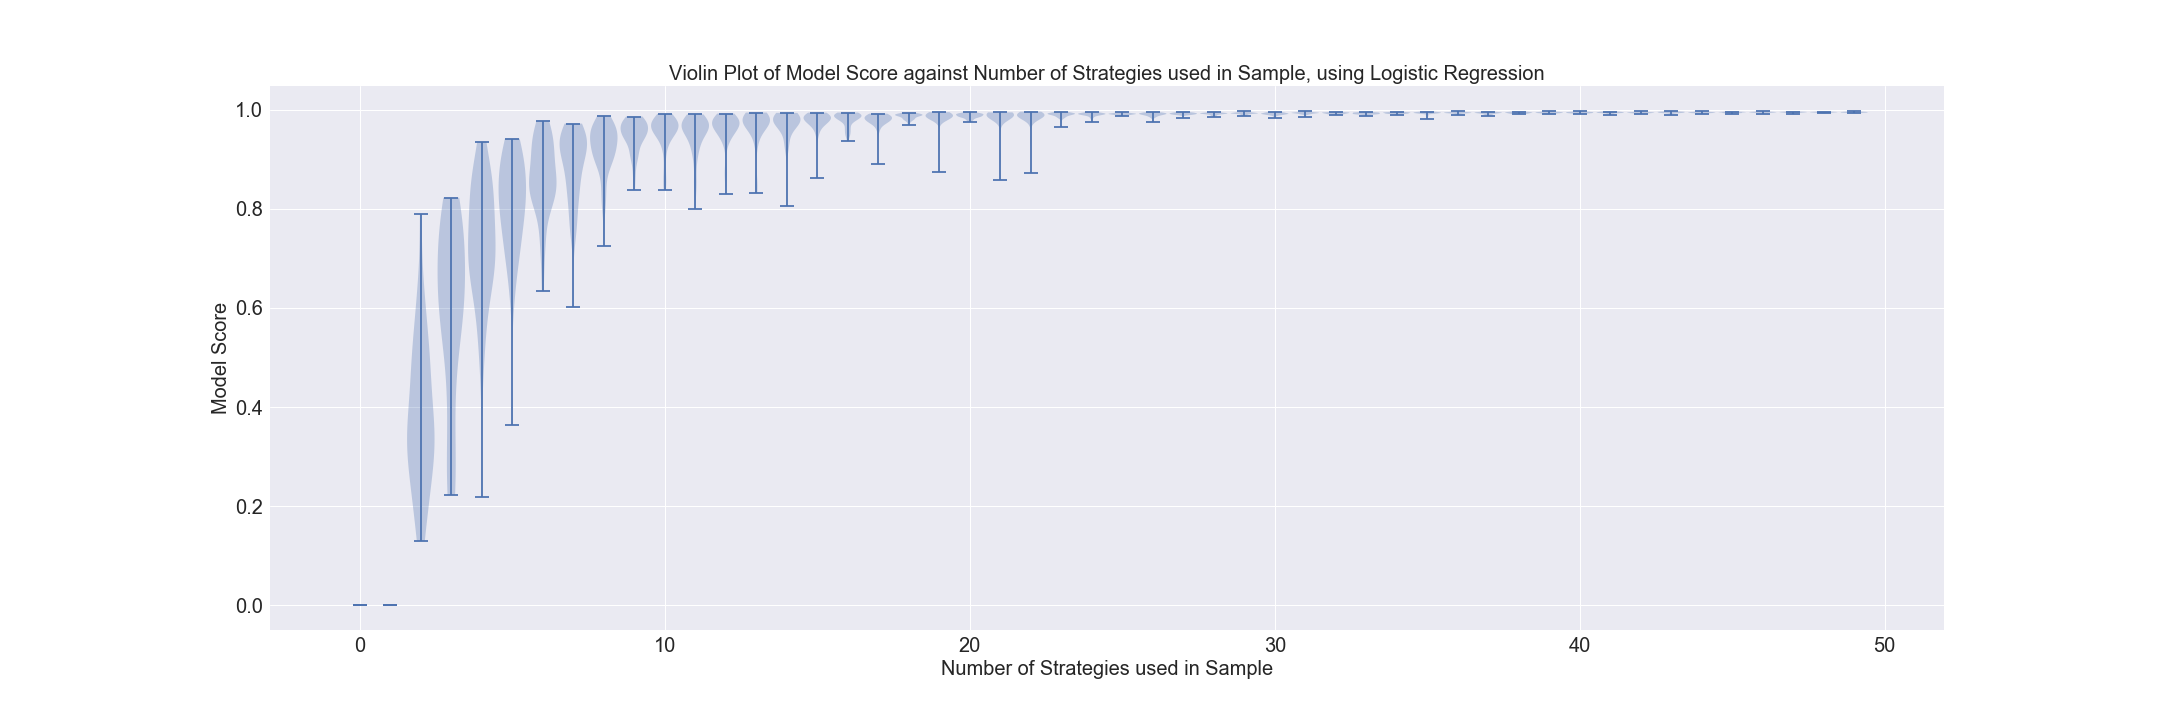
\includegraphics[width=\linewidth]{../img/ML/score_against_sample_size_LR.png}\label{fig:lr-samplesize}}\\
    \subfloat[Model performance against sample size for SVC]{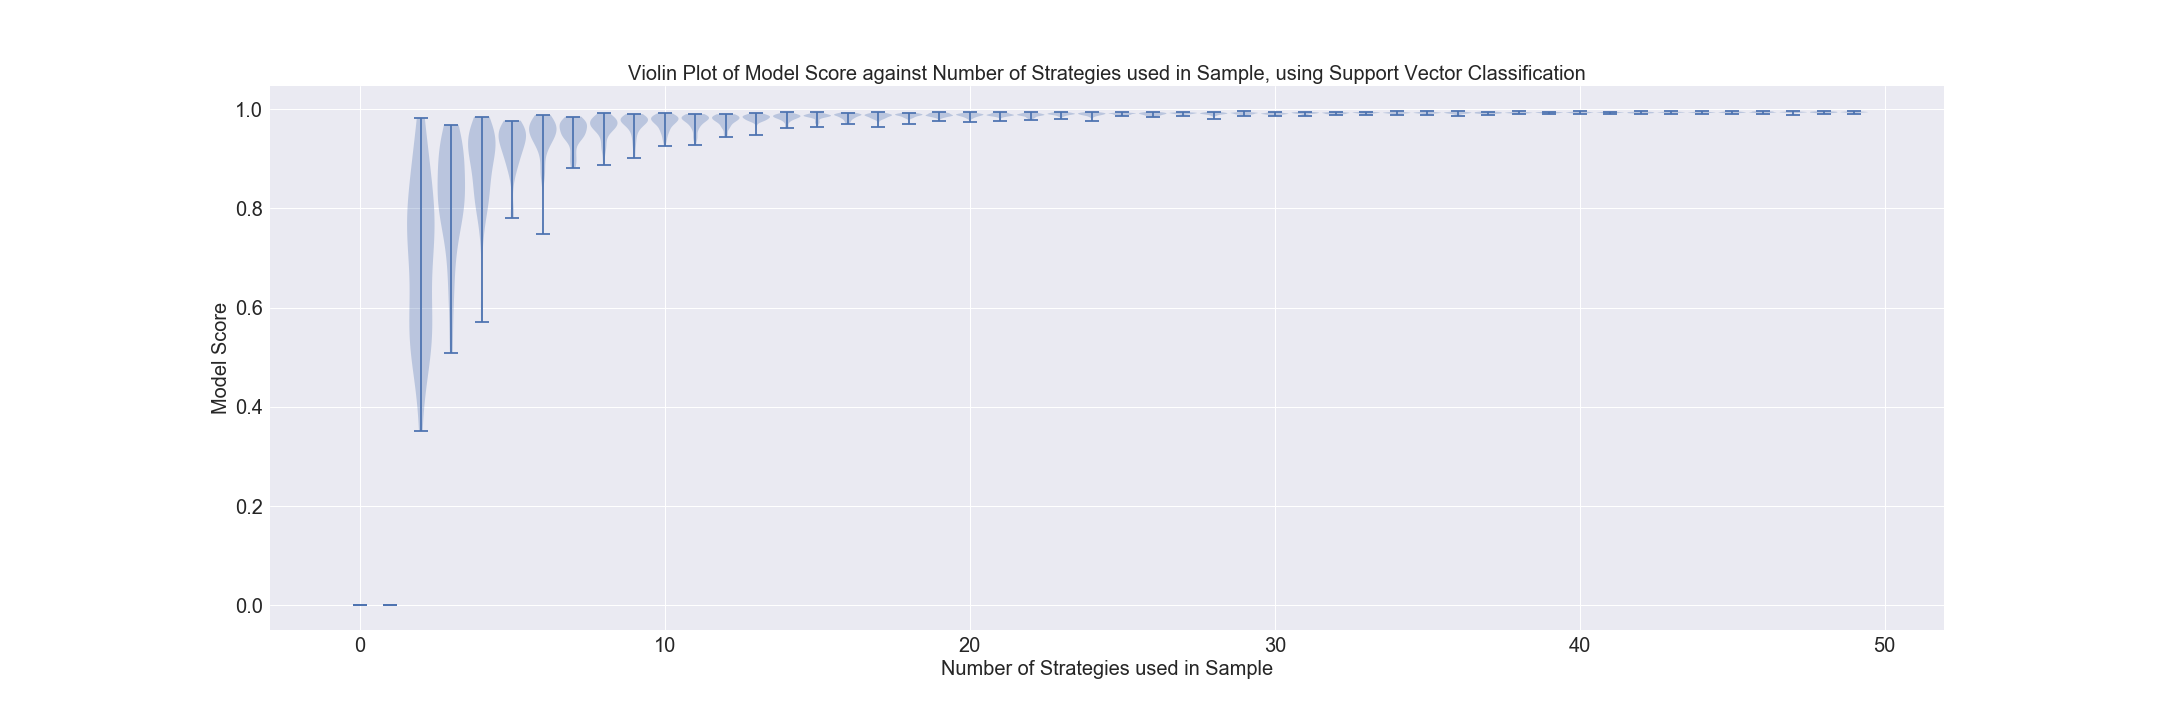
\includegraphics[width=\linewidth]{../img/ML/score_against_sample_size_SVC.png}\label{fig:svc-samplesize}}
    \caption{Violin Plots for both models}
    \label{fig:score_4_sample_size}
\end{figure}

It can be seen that the violins in Figure \ref{fig:svc-samplesize} reach a maximum score faster the those in Figure \ref{fig:lr-samplesize}.
Those is Figure \ref{fig:svc-samplesize} also show far less variance, and so the decision was made to use SVC as the model in any future work.
A sample size between 30 and 40 was deemed acceptable, due to a good balance between high score, low variance and computational cost.

The sample was chosen by analysing the results of the Round Robin Tournament in Axelrod-Python.
The strategies were ordered by their ranking in the tournament and every 5th one was selected.
This gave a balance of strategies that were similar (close ranking) and those that were very different (large difference in ranking).
Ordered by ranking, the 38 strategies chosen to train the model where:


\begin{multicols}{3}
\begin{enumerate}
  \item Evolved HMM 5
  \item Evolved ANN
  \item Evolved ANN 5 Noise 05
  \item PSO Gambler 2\_2\_2 Noise 05
  \item Nice Meta Winner Ensemble
  \item NMWE Long Memory
  \item EvolvedLookerUp1\_1\_1
  \item Shubik
  \item Retaliate (0.05)
  \item Soft Joss: 0.9
  \item GTFT: 0.3
  \item ShortMem
  \item Adaptive Pavlov 2011
  \item Punisher
  \item Grumpy
  \item Hard Tit For Tat
  \item Appeaser
  \item Meta Majority Finite Memory
  \item Average Copier
  \item Random Hunter
  \item Meta Hunter Aggressive
  \item Worse and Worse 2
  \item Predator
  \item Stochastic Cooperator
  \item Knowledgeable Worse and Worse
  \item Meta Winner Finite Memory
  \item Cautious QLearner
  \item Random: 0.1
  \item Meta Mixer
  \item EasyGo
  \item Hard Go By Majority: 40
  \item ZD-Extort-2 v2
  \item Opposite Grudger
  \item Alternator
  \item Tricky Defector
  \item Negation
  \item Gradual Killer
  \item Cycler CCCCCD
\end{enumerate}
\end{multicols}


\section{Initial Results}

%TODO confusion matrix

\begin{figure}[htbp!]
    \centering
    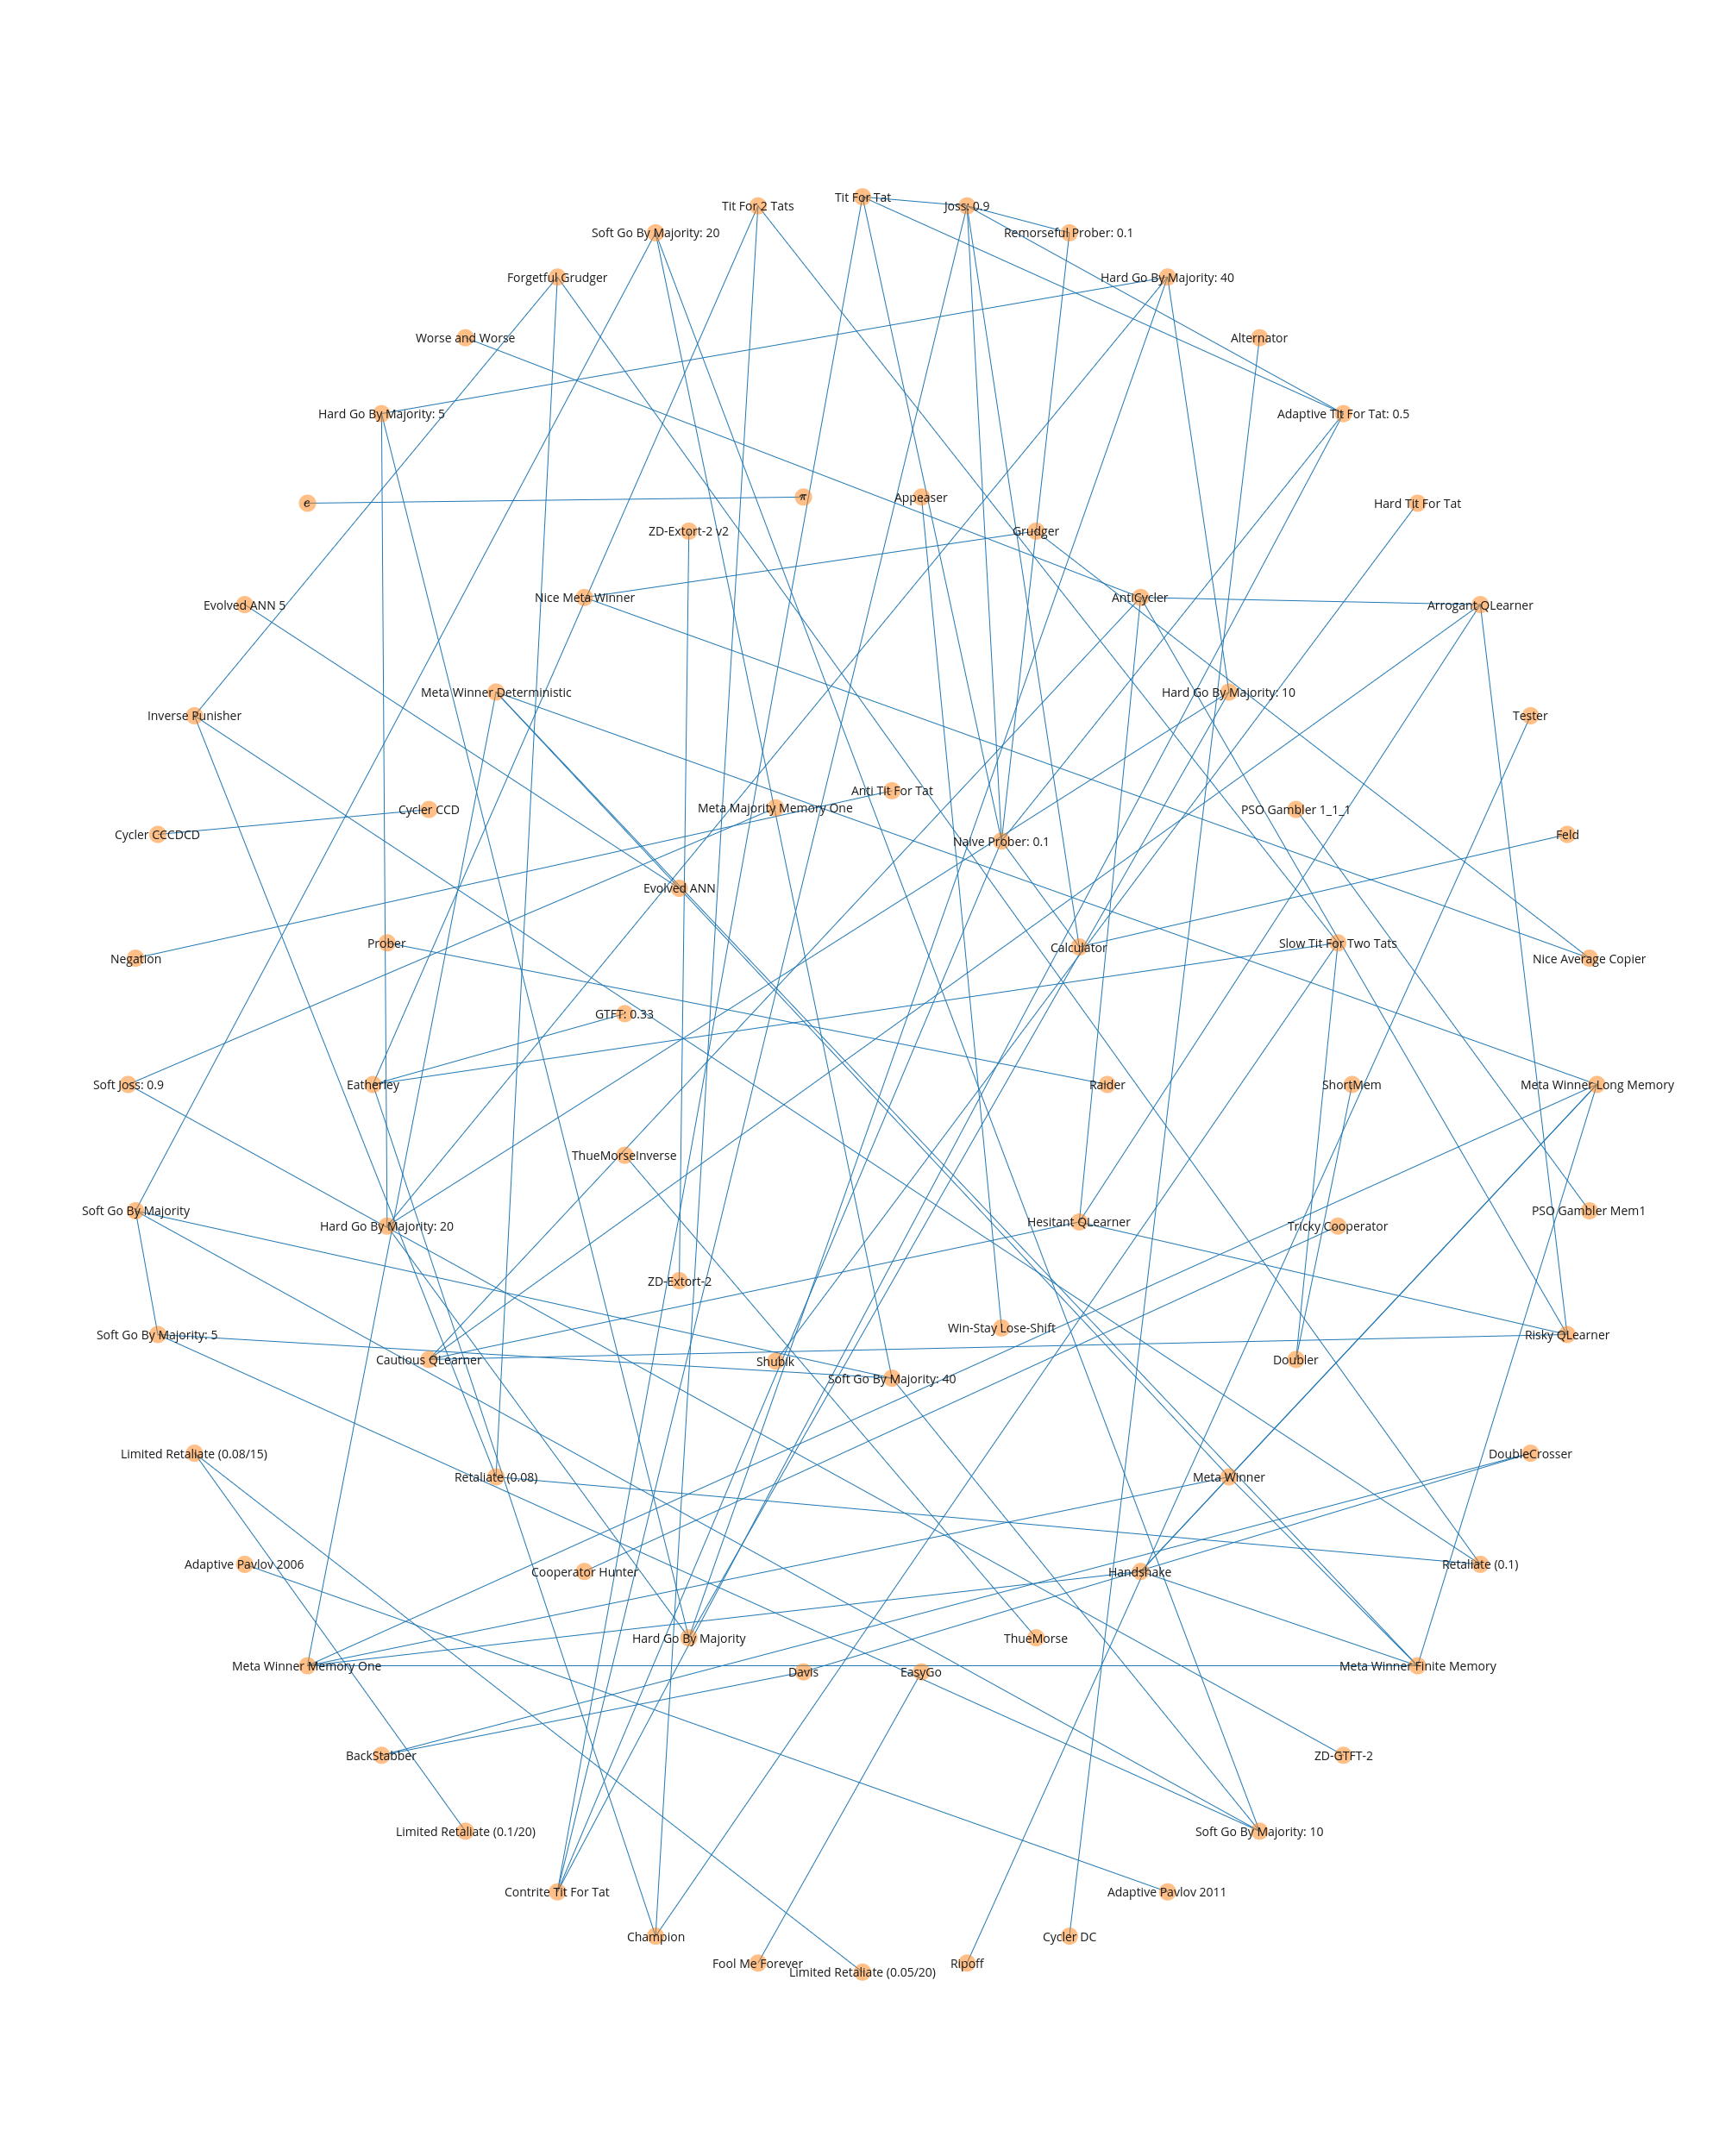
\includegraphics[width=\linewidth]{../img/neighbourhoods/overall.png}
    \caption{Caption here}
    \label{fig:figure1}
\end{figure}

% \begin{figure}[htbp!]
% \subfloat[]{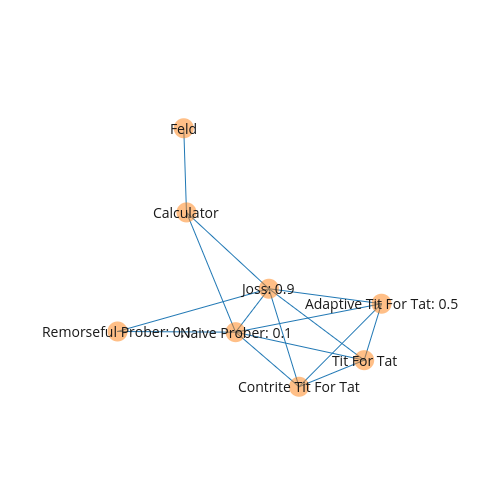
\includegraphics[width = 0.3\textwidth]{../img/neighbourhoods/1.png}}
% \subfloat[]{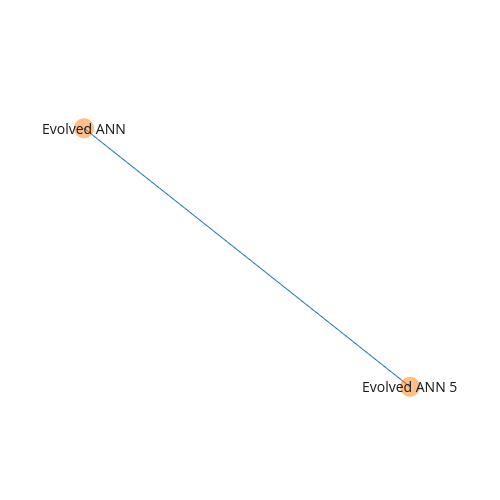
\includegraphics[width = 0.3\textwidth]{../img/neighbourhoods/2.png}}
% \subfloat[]{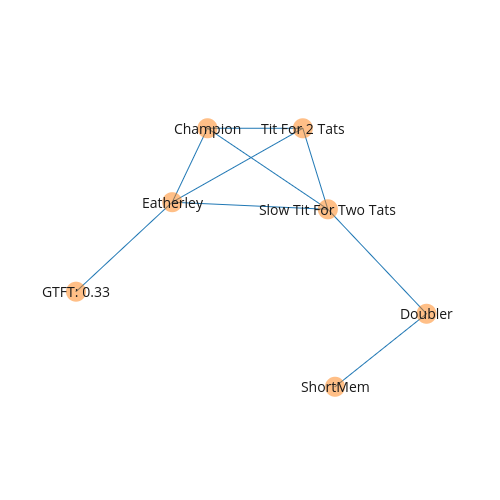
\includegraphics[width = 0.3\textwidth]{../img/neighbourhoods/3.png}} \\
% \end{figure}
% \begin{figure}[htbp!]
% \ContinuedFloat
% \subfloat[]{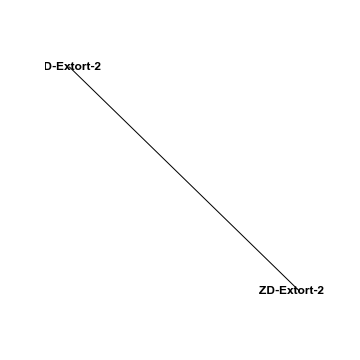
\includegraphics[width = 0.3\textwidth]{../img/neighbourhoods/4.png}}
% \subfloat[]{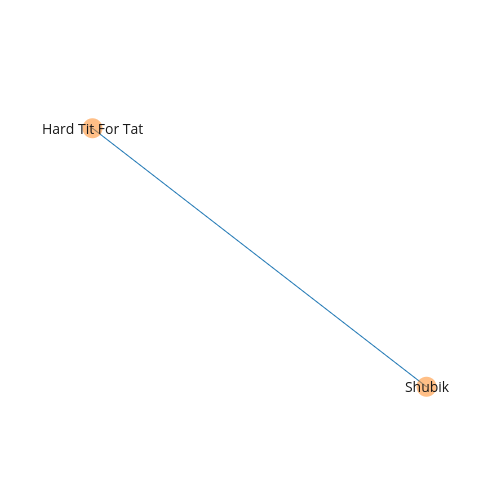
\includegraphics[width = 0.3\textwidth]{../img/neighbourhoods/5.png}}
% \subfloat[]{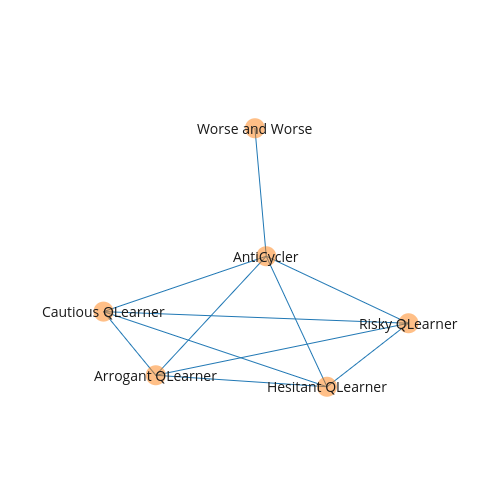
\includegraphics[width = 0.3\textwidth]{../img/neighbourhoods/6.png}} \\
% \end{figure}
% \begin{figure}[htbp!]
% \ContinuedFloat
% \subfloat[]{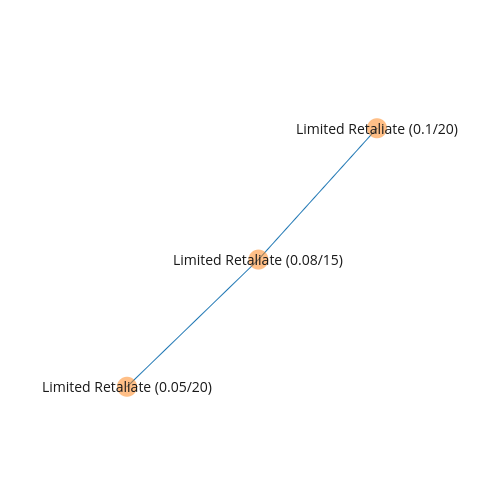
\includegraphics[width = 0.3\textwidth]{../img/neighbourhoods/7.png}}
% \subfloat[]{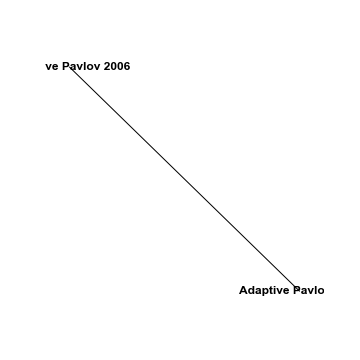
\includegraphics[width = 0.3\textwidth]{../img/neighbourhoods/8.png}}
% \subfloat[]{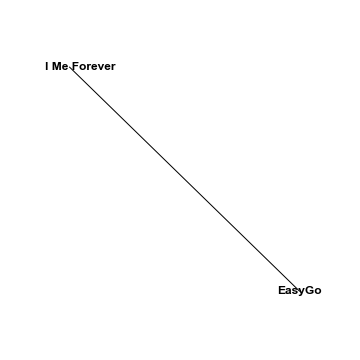
\includegraphics[width = 0.3\textwidth]{../img/neighbourhoods/9.png}} \\
% \end{figure}
% \begin{figure}[htbp!]
% \ContinuedFloat
% \subfloat[]{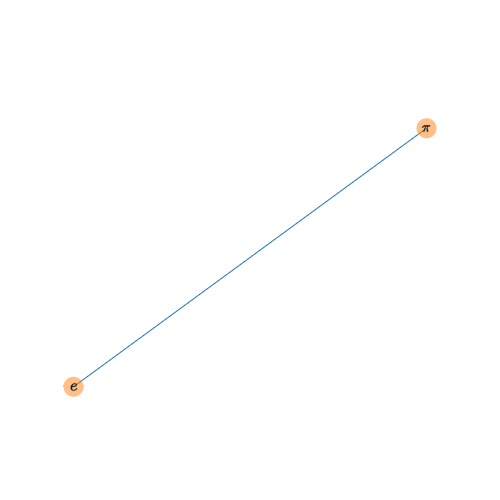
\includegraphics[width = 0.3\textwidth]{../img/neighbourhoods/10.png}}
% \subfloat[]{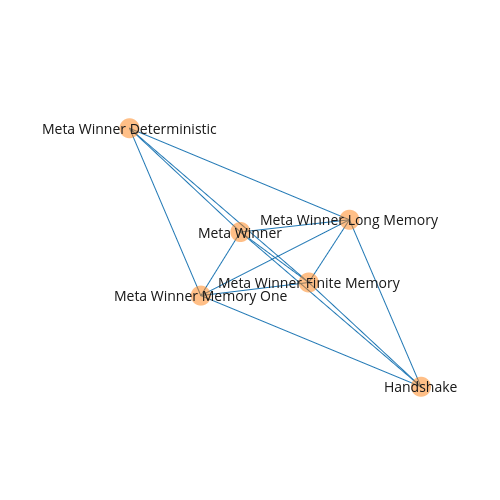
\includegraphics[width = 0.3\textwidth]{../img/neighbourhoods/11.png}}
% \subfloat[]{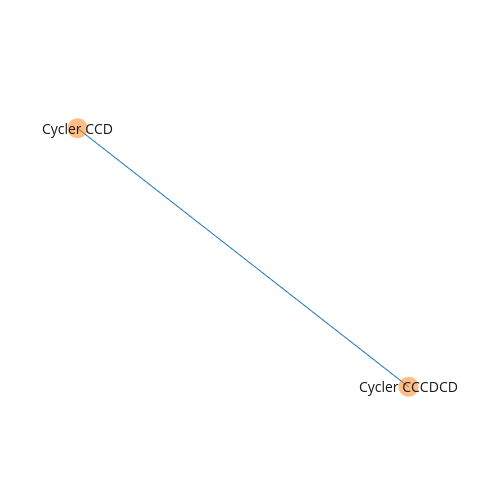
\includegraphics[width = 0.3\textwidth]{../img/neighbourhoods/12.png}} \\
% \end{figure}
% \begin{figure}[htbp!]
% \ContinuedFloat
% \subfloat[]{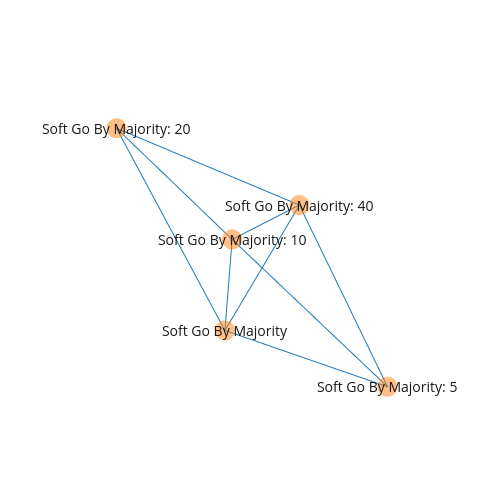
\includegraphics[width = 0.3\textwidth]{../img/neighbourhoods/13.png}}
% \subfloat[]{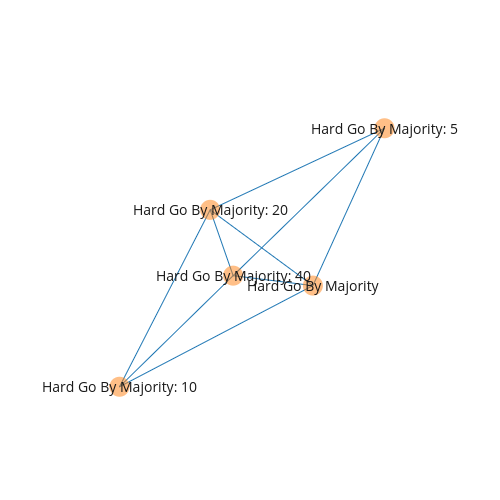
\includegraphics[width = 0.3\textwidth]{../img/neighbourhoods/14.png}}
% \subfloat[]{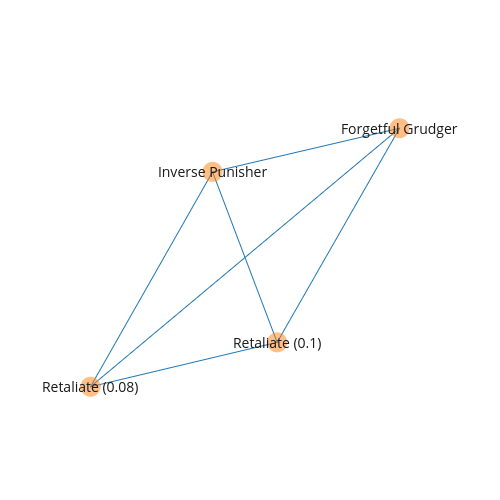
\includegraphics[width = 0.3\textwidth]{../img/neighbourhoods/15.png}} \\
% \end{figure}
% \begin{figure}[htbp!]
% \ContinuedFloat
% \subfloat[]{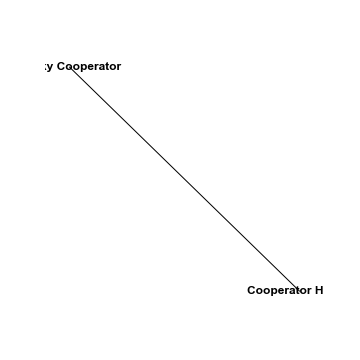
\includegraphics[width = 0.3\textwidth]{../img/neighbourhoods/16.png}}
% \subfloat[]{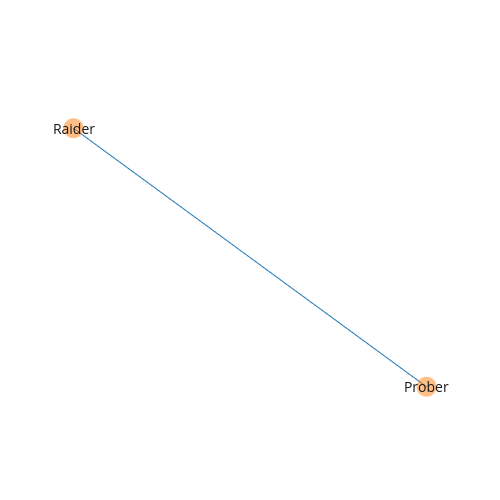
\includegraphics[width = 0.3\textwidth]{../img/neighbourhoods/17.png}}
% \subfloat[]{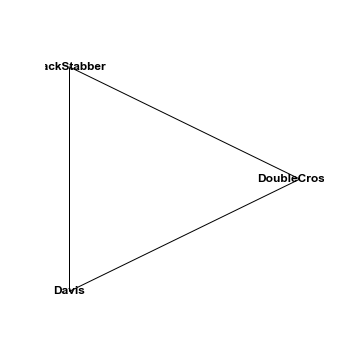
\includegraphics[width = 0.3\textwidth]{../img/neighbourhoods/18.png}} \\
% \end{figure}
% \begin{figure}[htbp!]
% \ContinuedFloat
% \subfloat[]{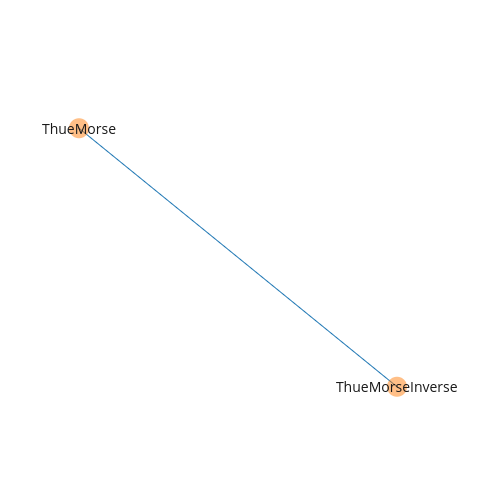
\includegraphics[width = 0.3\textwidth]{../img/neighbourhoods/19.png}}
% \subfloat[]{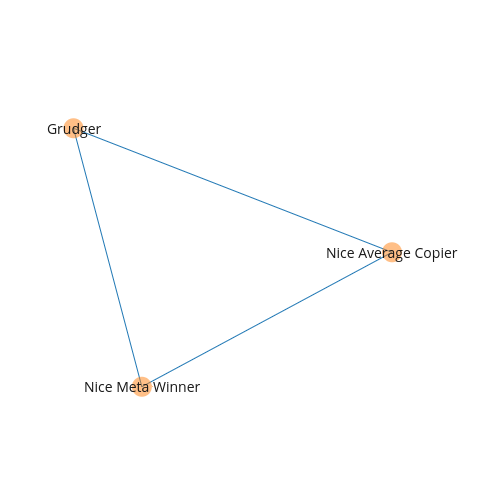
\includegraphics[width = 0.3\textwidth]{../img/neighbourhoods/20.png}}
% \subfloat[]{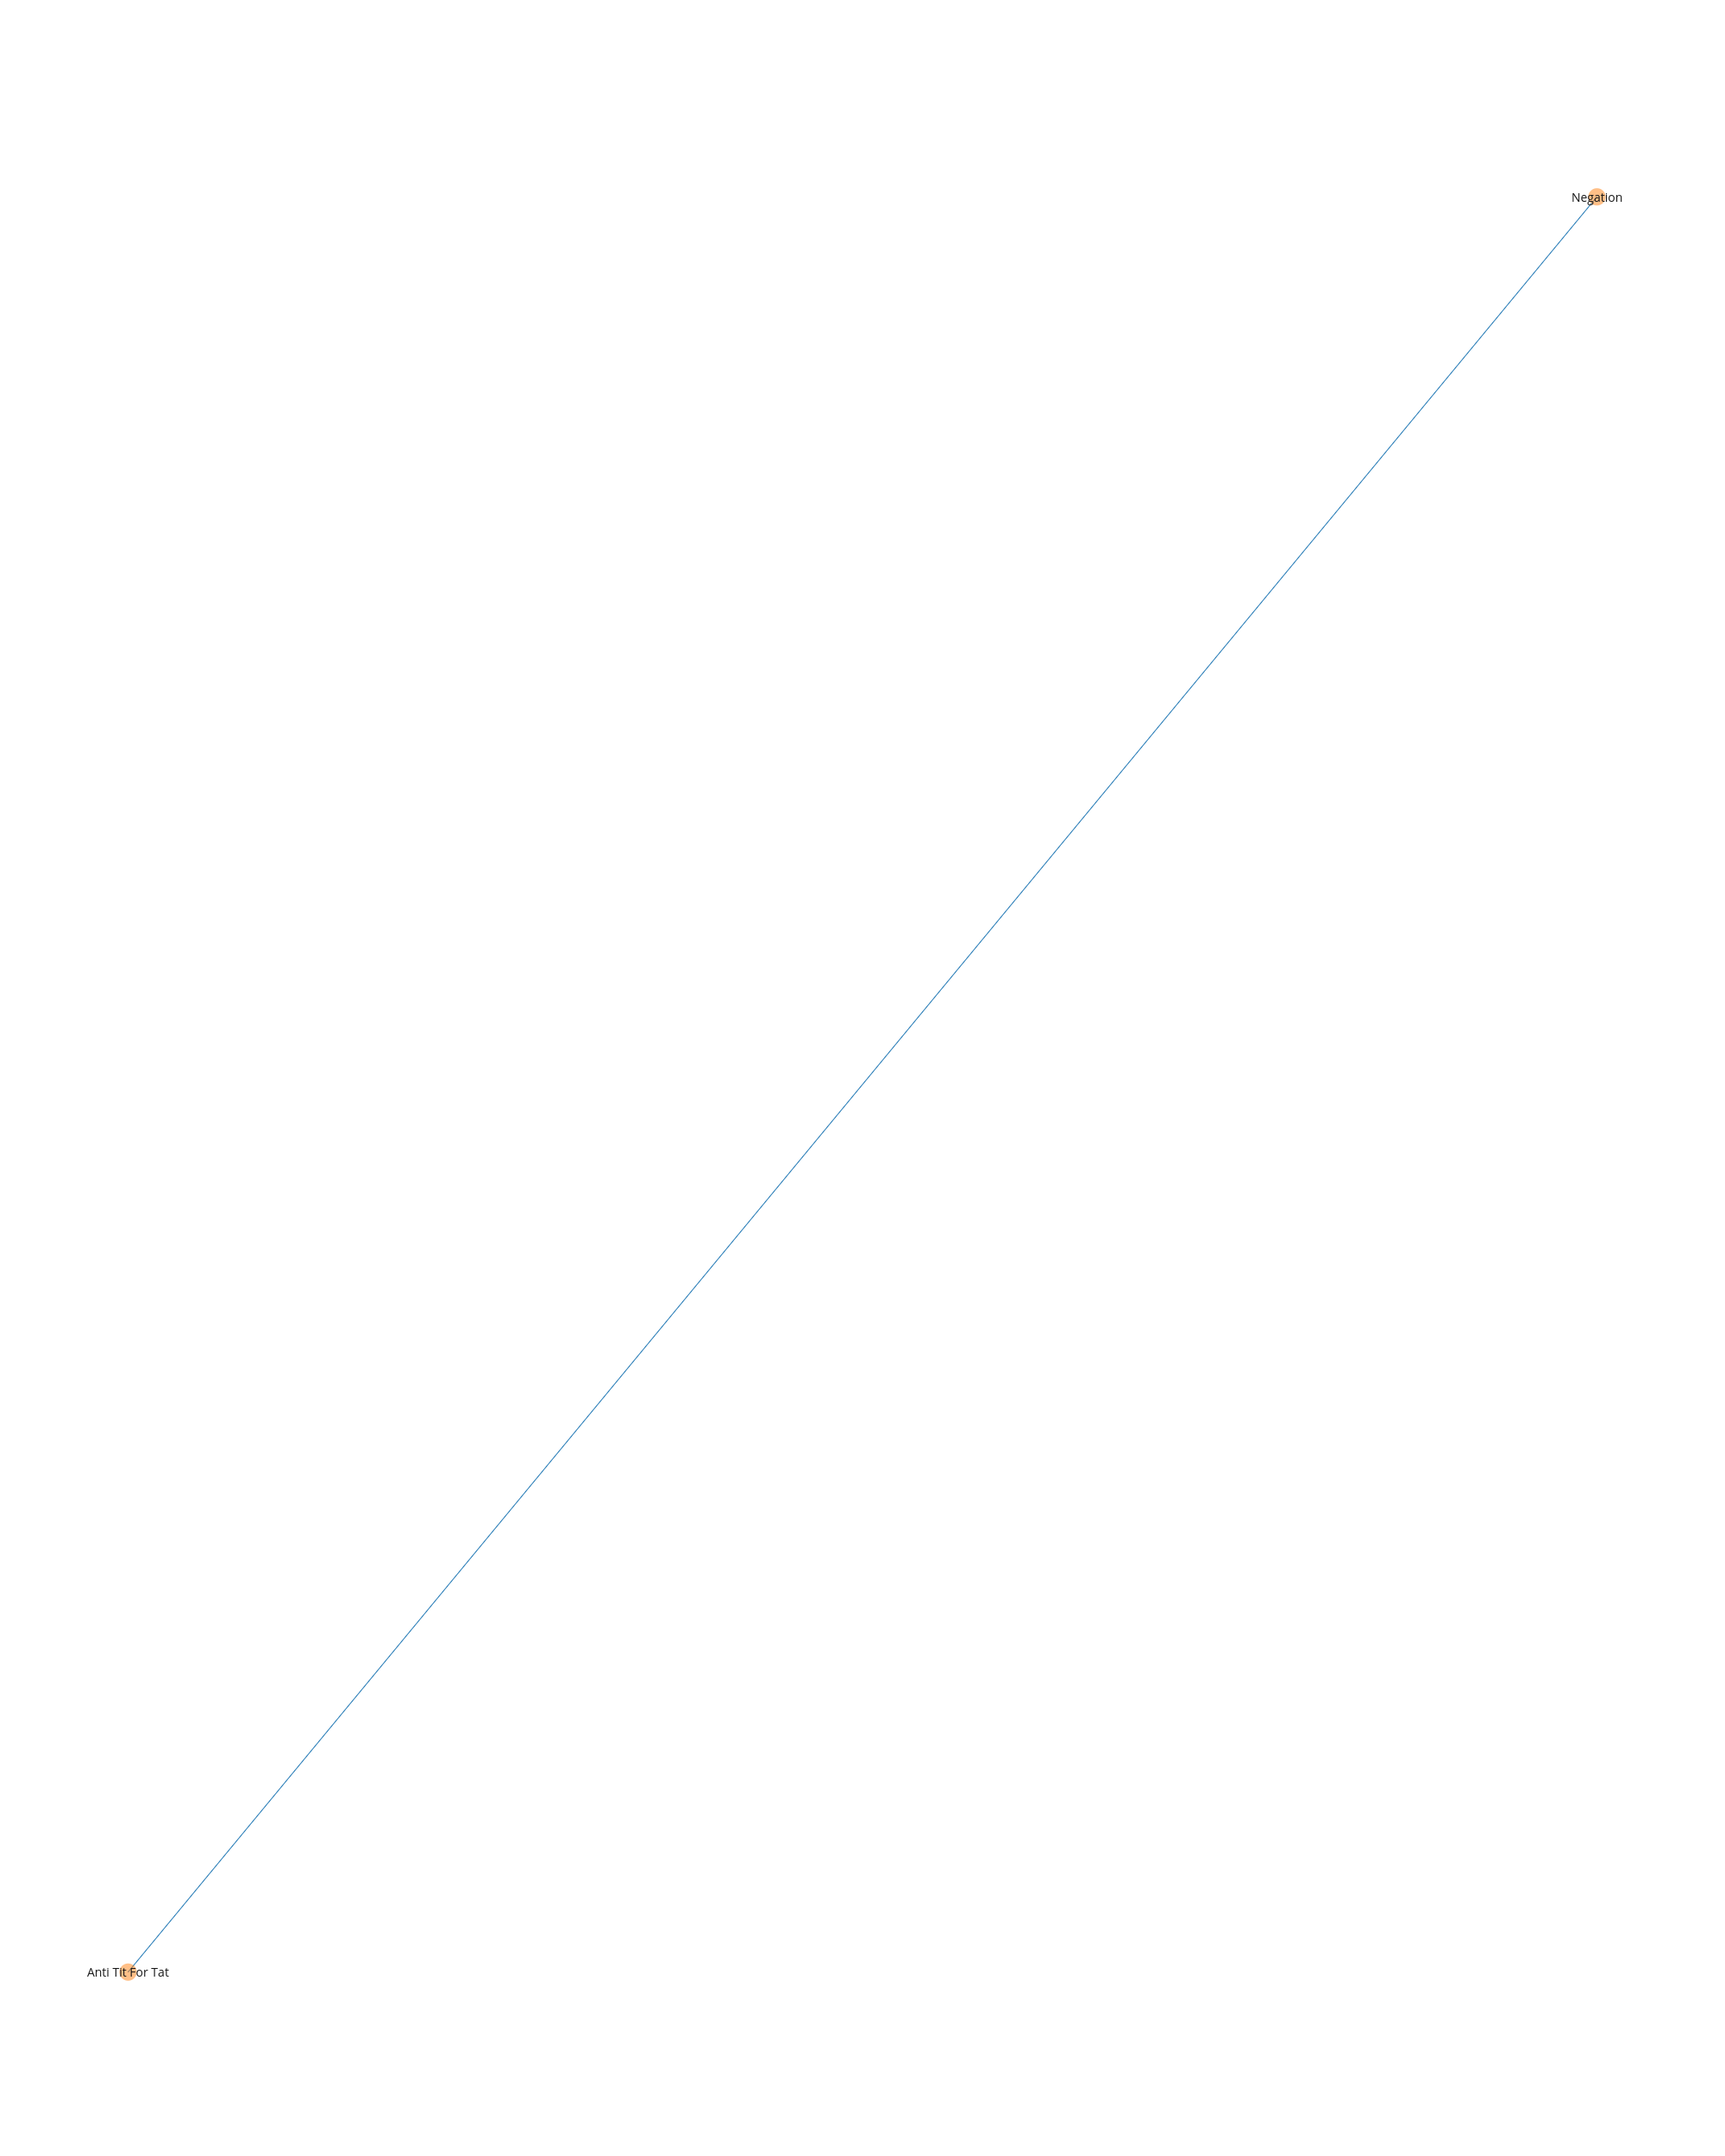
\includegraphics[width = 0.3\textwidth]{../img/neighbourhoods/21.png}} \\
% \end{figure}
% \begin{figure}[htbp!]
% \ContinuedFloat
% \subfloat[]{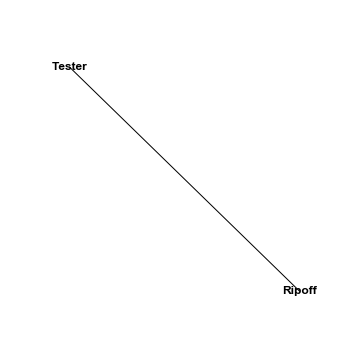
\includegraphics[width = 0.3\textwidth]{../img/neighbourhoods/22.png}}
% \subfloat[]{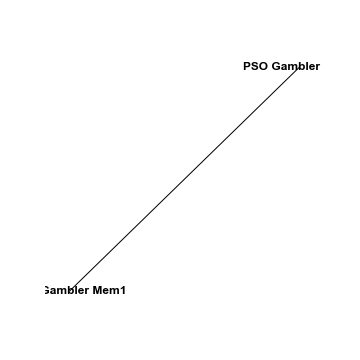
\includegraphics[width = 0.3\textwidth]{../img/neighbourhoods/23.png}}
% \subfloat[]{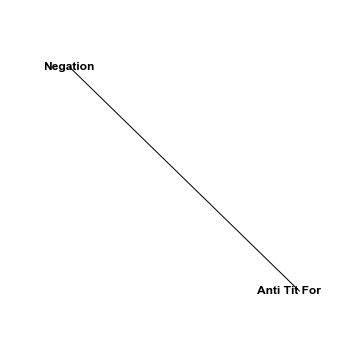
\includegraphics[width = 0.3\textwidth]{../img/neighbourhoods/24.png}} \\
% \end{figure}
% \begin{figure}[htbp!]
% \ContinuedFloat
% \subfloat[]{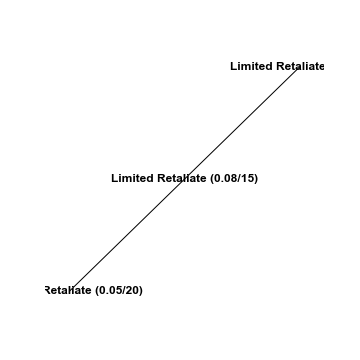
\includegraphics[width = 0.3\textwidth]{../img/neighbourhoods/25.png}}
% \subfloat[]{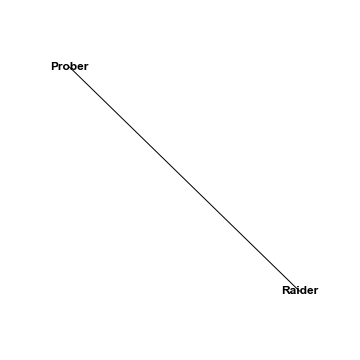
\includegraphics[width = 0.3\textwidth]{../img/neighbourhoods/0.png}}\\
% \end{figure}
